% Options for packages loaded elsewhere
\PassOptionsToPackage{unicode}{hyperref}
\PassOptionsToPackage{hyphens}{url}
%
\documentclass[
]{article}
\usepackage{amsmath,amssymb}
\usepackage{lmodern}
\usepackage{ifxetex,ifluatex}
\ifnum 0\ifxetex 1\fi\ifluatex 1\fi=0 % if pdftex
  \usepackage[T1]{fontenc}
  \usepackage[utf8]{inputenc}
  \usepackage{textcomp} % provide euro and other symbols
\else % if luatex or xetex
  \usepackage{unicode-math}
  \defaultfontfeatures{Scale=MatchLowercase}
  \defaultfontfeatures[\rmfamily]{Ligatures=TeX,Scale=1}
  \setsansfont[]{Calibri Light}
\fi
% Use upquote if available, for straight quotes in verbatim environments
\IfFileExists{upquote.sty}{\usepackage{upquote}}{}
\IfFileExists{microtype.sty}{% use microtype if available
  \usepackage[]{microtype}
  \UseMicrotypeSet[protrusion]{basicmath} % disable protrusion for tt fonts
}{}
\makeatletter
\@ifundefined{KOMAClassName}{% if non-KOMA class
  \IfFileExists{parskip.sty}{%
    \usepackage{parskip}
  }{% else
    \setlength{\parindent}{0pt}
    \setlength{\parskip}{6pt plus 2pt minus 1pt}}
}{% if KOMA class
  \KOMAoptions{parskip=half}}
\makeatother
\usepackage{xcolor}
\IfFileExists{xurl.sty}{\usepackage{xurl}}{} % add URL line breaks if available
\IfFileExists{bookmark.sty}{\usepackage{bookmark}}{\usepackage{hyperref}}
\hypersetup{
  pdftitle={SDS Project},
  pdfauthor={G. Cristiano, R. Incandela, N. Karani},
  hidelinks,
  pdfcreator={LaTeX via pandoc}}
\urlstyle{same} % disable monospaced font for URLs
\usepackage[margin=1in]{geometry}
\usepackage{graphicx}
\makeatletter
\def\maxwidth{\ifdim\Gin@nat@width>\linewidth\linewidth\else\Gin@nat@width\fi}
\def\maxheight{\ifdim\Gin@nat@height>\textheight\textheight\else\Gin@nat@height\fi}
\makeatother
% Scale images if necessary, so that they will not overflow the page
% margins by default, and it is still possible to overwrite the defaults
% using explicit options in \includegraphics[width, height, ...]{}
\setkeys{Gin}{width=\maxwidth,height=\maxheight,keepaspectratio}
% Set default figure placement to htbp
\makeatletter
\def\fps@figure{htbp}
\makeatother
\setlength{\emergencystretch}{3em} % prevent overfull lines
\providecommand{\tightlist}{%
  \setlength{\itemsep}{0pt}\setlength{\parskip}{0pt}}
\setcounter{secnumdepth}{-\maxdimen} % remove section numbering
\usepackage{booktabs}
\usepackage{longtable}
\usepackage{array}
\usepackage{multirow}
\usepackage{wrapfig}
\usepackage{float}
\usepackage{colortbl}
\usepackage{pdflscape}
\usepackage{tabu}
\usepackage{threeparttable}
\usepackage{threeparttablex}
\usepackage[normalem]{ulem}
\usepackage{makecell}
\usepackage{xcolor}
\ifluatex
  \usepackage{selnolig}  % disable illegal ligatures
\fi

\title{SDS Project}
\author{G. Cristiano, R. Incandela, N. Karani}
\date{3/25/2021}

\begin{document}
\maketitle

\fontsize{11}{14}
\selectfont

\hypertarget{list-of-countries-of-interest}{%
\subsection{List of countries of
interest}\label{list-of-countries-of-interest}}

We consider all European countries: Austria, Belgium, Bulgaria,
Switzerland, Cyprus, Czech Republic, Germany, Denmark, Spain, Estonia,
Finland, France, United Kingdom, Greece, Croatia, Hungary, Iceland,
Italy, Lithuania, Luxembourg, Latvia, Malta, Netherlands, Norway,
Poland, Portugal, Romania, Slovakia, Slovenia and Sweden. The ISO
country codes can be searched from
\url{https://www.iban.com/country-codes}.

\hypertarget{time-period-of-interest}{%
\subsection{Time period of interest}\label{time-period-of-interest}}

In order to keep the time period consistent between the world bank and
the LinkedIn data, we choose the time period of interest from 2015 to
2019.

\hypertarget{economic-indicators-of-interest}{%
\subsection{Economic indicators of
interest}\label{economic-indicators-of-interest}}

For these indicators, we extract the data from the world bank interface.
The entire list of indicators can be seen here:
\url{https://databank.worldbank.org/source/world-development-indicators}.

First, we need the GDP per capita. This is the main variable of
interest. For the analyses, we consider this as the dependent variable,
and seek to understand the effect of various unemployment related
parameters on the GDP per capita. There are several indicators of GDP
per capital: constant 2010 US dollars, current US dollars, constant LCU,
current LCU, etc. We use the GDP per capita in constant 2010 US dollars
for our analysis.

Among the unemployment indicators, we consider (i) the total
unemployment percentage, (ii) the unemployment percentage in youths
(ages 15-24), (iii) the unemployment percentage among males, and (iv)
the unemployment percentage among females. In the world bank interface,
for all these indicators, we have two estimates: (i) a national estimate
and (ii) a modeled ILO estimate. For our analysis, we consider the
national estimate.

Finally, we consider the division of the total employment in different
industry sectors: namely (i) agriculture (consisting of activities in
agriculture, hunting, forestry and fishing), (ii) industry (consisting
of mining and quarrying, manufacturing, construction, and public
utilities (electricity, gas, and water) and (iii) services (consisting
of wholesale and retail trade and restaurants and hotels; transport,
storage, and communications; financing, insurance, real estate, and
business services; and community, social, and personal services). For
these indicators, only one estimate (the modeled ILO estimate) is
available, and we use the same.

\hypertarget{correlation-between-total-unemployment-and-gdp-per-capita-2015---2019}{%
\subsection{Correlation between total unemployment and GDP per capita
(2015 -
2019)}\label{correlation-between-total-unemployment-and-gdp-per-capita-2015---2019}}

The Pearson correlation coefficient between the total unemployment rate
and the per capita GDP between 2015 and 2019 in European countries is
-0.186.

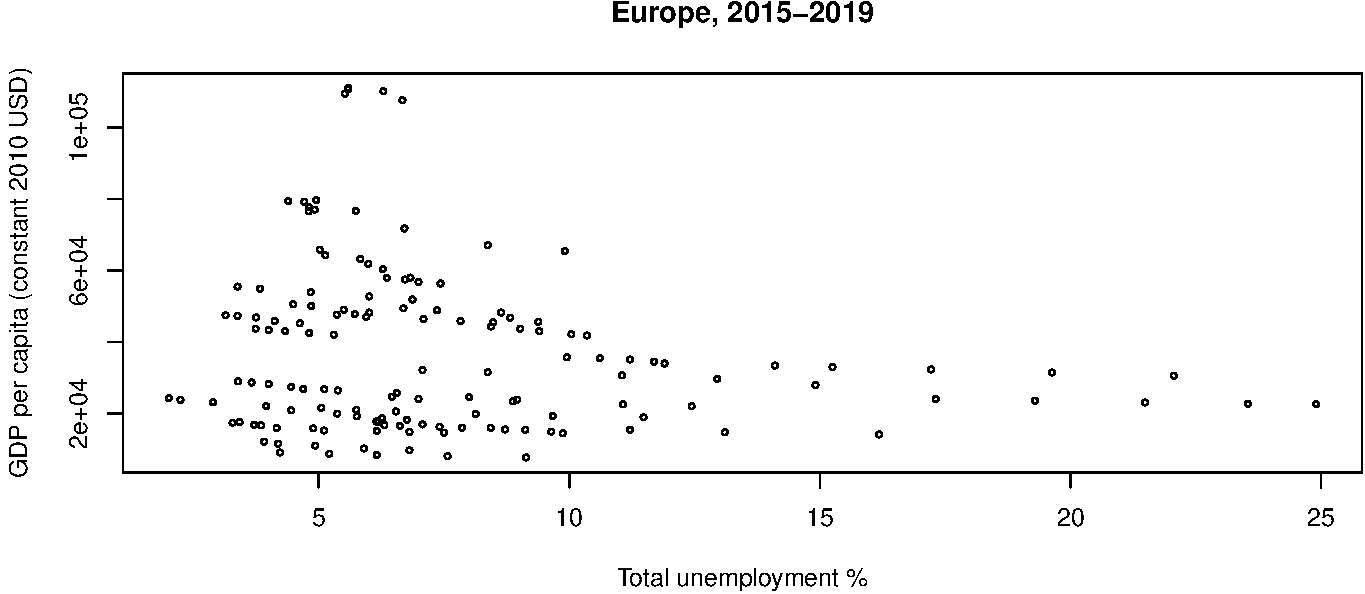
\includegraphics{main_files/figure-latex/unnamed-chunk-7-1.pdf}

In order to check the statistical significance of the computed
correlation, let's do a permutation analysis. Taking \ensuremath{10^{4}}
permutations, we find the p-value of the measured correlation to be
0.0071. As the p-value is smaller than 0.05, the measured correlation is
statistically significant.

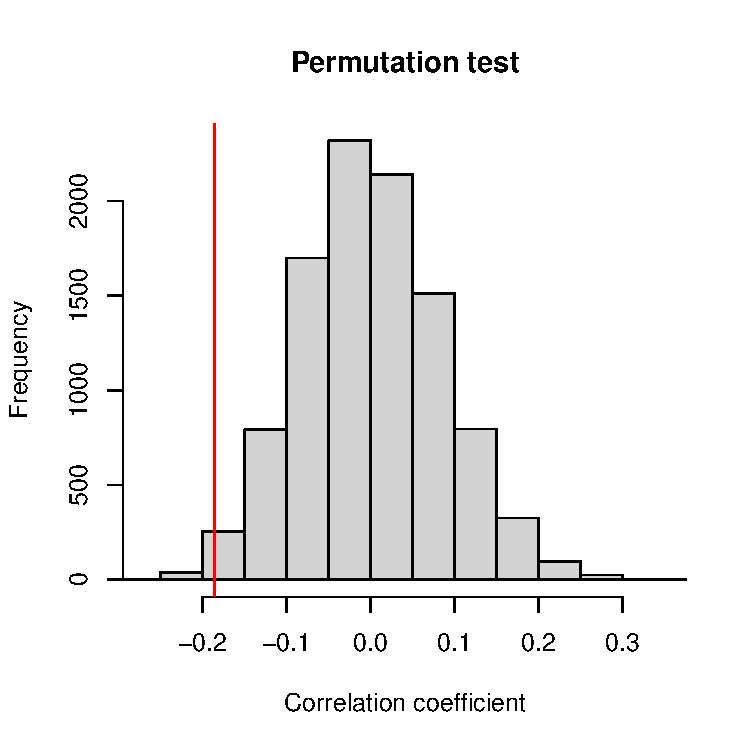
\includegraphics{main_files/figure-latex/permutation_plot-1.pdf}

Further, let's do a bootstrap analysis to quantify the uncertainty in
the measured correlation value. Repeating the bootstrap analysis
\ensuremath{10^{4}} times, we find the mean correlation to be -0.185,
with a standard deviation of 0.0429. Thus, although the measured
coefficient is unbiased, there seems to relatively high uncertainty in
the measurement. This shows the unreliability of the measured
correlation, and indicates that the real correlation value for a larger
data-set may be remarkably different.

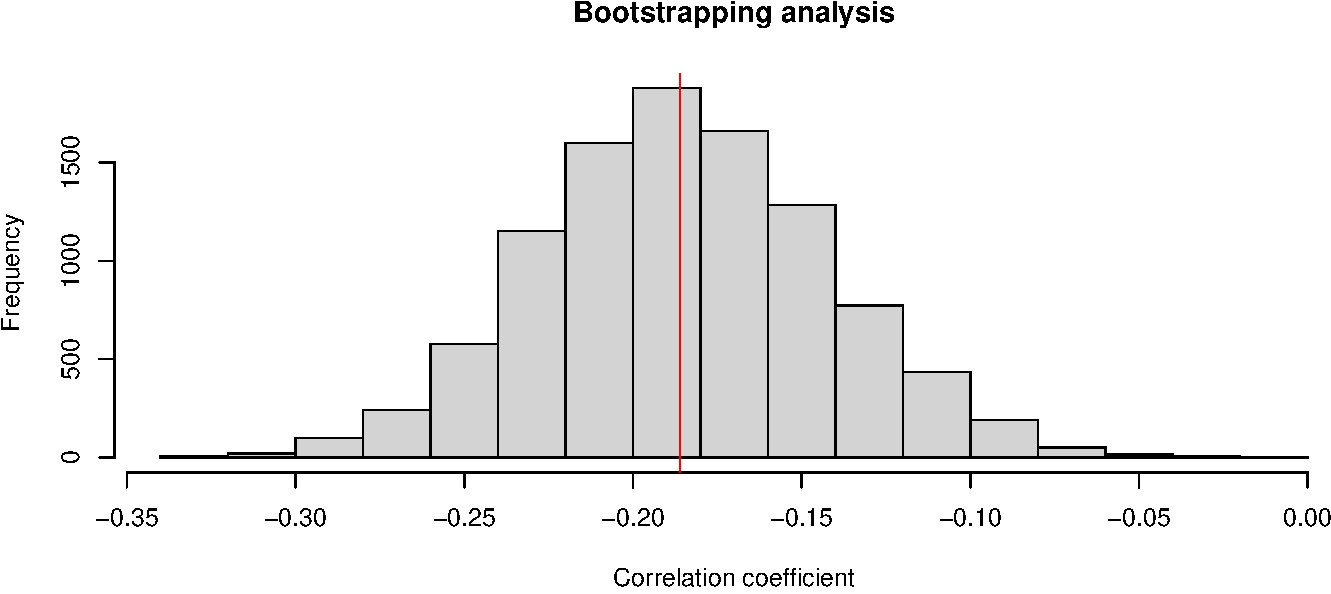
\includegraphics{main_files/figure-latex/unnamed-chunk-8-1.pdf}

\hypertarget{yearwise-analysis-2005---2019}{%
\subsection{Yearwise analysis (2005 -
2019)}\label{yearwise-analysis-2005---2019}}

The substantial uncertainty in the measured correlation could be due to
multiple reasons. It may indicate that the relationship between the GDP
per capita and the total unemployment is complicated, and perhaps
dependent on several other variables. Further, the cumulative analysis
over the 5 year time period (2015 - 2019) may be further complicating
the relationship by introducing additional variations that may have
occurred in different countries in different years within the considered
time period. In order to alleviate this complication, we study the
relationship between the GDP per capita and the total unemployment for
each year separately. As there is no dependency of this yearwise
analysis on the LinkedIN analysis, and to benefit from the additional
data available via the WDI interface, we include an extended time
period: from 2005 to 2019.

\begin{verbatim}
## [1] "Year | Correlation | BT mean | BT std | p-value"
\end{verbatim}

\begin{verbatim}
## [1] "2005 -0.562 -0.57 0.0812 2e-04"
## [1] "2006 -0.517 -0.518 0.1 6e-04"
## [1] "2007 -0.458 -0.452 0.126 0.0045"
## [1] "2008 -0.37 -0.372 0.125 0.0202"
## [1] "2009 -0.428 -0.43 0.129 0.0041"
## [1] "2010 -0.509 -0.51 0.113 9e-04"
## [1] "2011 -0.494 -0.503 0.118 0.0019"
## [1] "2012 -0.441 -0.456 0.115 0.0041"
## [1] "2013 -0.398 -0.413 0.107 0.0053"
## [1] "2014 -0.347 -0.357 0.103 0.0163"
## [1] "2015 -0.275 -0.282 0.0999 0.0536"
## [1] "2016 -0.224 -0.226 0.0994 0.1069"
## [1] "2017 -0.181 -0.178 0.105 0.1755"
## [1] "2018 -0.115 -0.107 0.103 0.2954"
## [1] "2019 -0.0647 -0.0501 0.112 0.4112"
\end{verbatim}

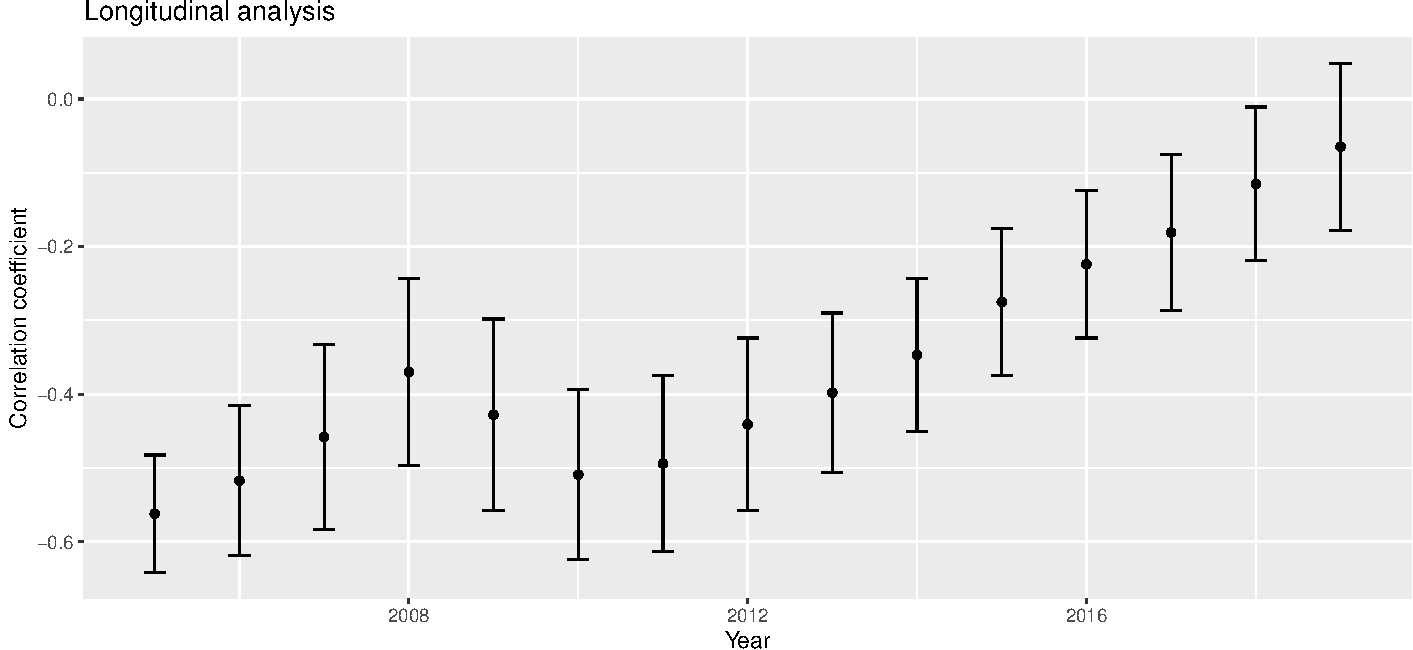
\includegraphics{main_files/figure-latex/correlation_one_year-1.pdf}

We observe a clear trend in the yearwise analysis: the correlation
between the total unemployment and the GDP per capita becomes
consistently weaker from 2010 to 2019. The error bars in the plot above
indicate the standard deviation values computed via bootstrapping.
Further, permutation testing shows that the correlation values before
2016 are statistically significant, while the ones from 2016 are not.

Based on this analysis, we conclude that there may be several
time-dependent factors affecting the relationship between the GDP per
capita and the total unemployment. A multivariate analysis including
such additional factors is outside the scope of this project.
Accordingly, we decide to focus on a single year for the further
analysis. As the correlation is statistically significant before 2016,
and we have LinkedIn data available from 2015 onwards, 2015 is the only
year which matches both our analysis criteria.

\hypertarget{group-analysis-2015}{%
\subsection{Group Analysis (2015)}\label{group-analysis-2015}}

The table below shows the correlation values for different sub-groups in
the population. It can be seen that the correlation values are quite
similar for all the considered groups.

\begin{table}
\centering
\begin{tabular}{l|r|r|r|r}
\hline
  & Correlation & Bootstrapping mean & Bootstrapping std. dev. & P-value\\
\hline
Total & -0.275 & -0.276 & 0.0400 & 0.0571\\
\hline
Youth & -0.287 & -0.288 & 0.0423 & 0.0553\\
\hline
Male & -0.296 & -0.296 & 0.0445 & 0.0452\\
\hline
Female & -0.251 & -0.253 & 0.0377 & 0.0729\\
\hline
\end{tabular}
\end{table}

\hypertarget{mediation-analysis-2015}{%
\subsection{Mediation Analysis (2015)}\label{mediation-analysis-2015}}

\hypertarget{dataframe-merging}{%
\section{Dataframe merging}\label{dataframe-merging}}

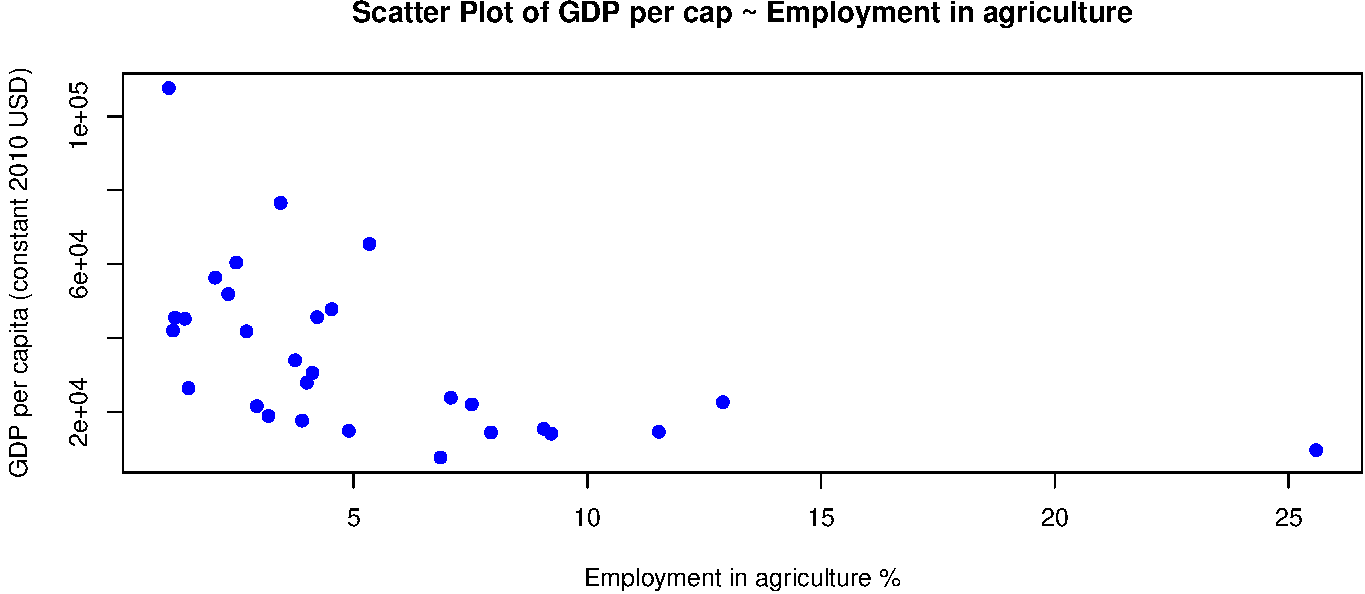
\includegraphics{main_files/figure-latex/mediation_agr-1.pdf}

\begin{table}
\centering
\begin{tabular}{l|r|r|r|r|r|r}
\hline
  & I->D & p-value & I->M & p-value & ACME & p-value\\
\hline
Youth & -2330.969 & 0.0050255 & 0.6402022 & 0.1435720 & -202.9785 & 0.294\\
\hline
Female & -2330.969 & 0.0050255 & 0.2482897 & 0.2463356 & -149.0624 & 0.622\\
\hline
\end{tabular}
\end{table}

\hypertarget{mediation-analysis-gdp-unemp_youth-empl_ind}{%
\section{Mediation analysis (GDP, unemp\_youth,
empl\_ind)}\label{mediation-analysis-gdp-unemp_youth-empl_ind}}

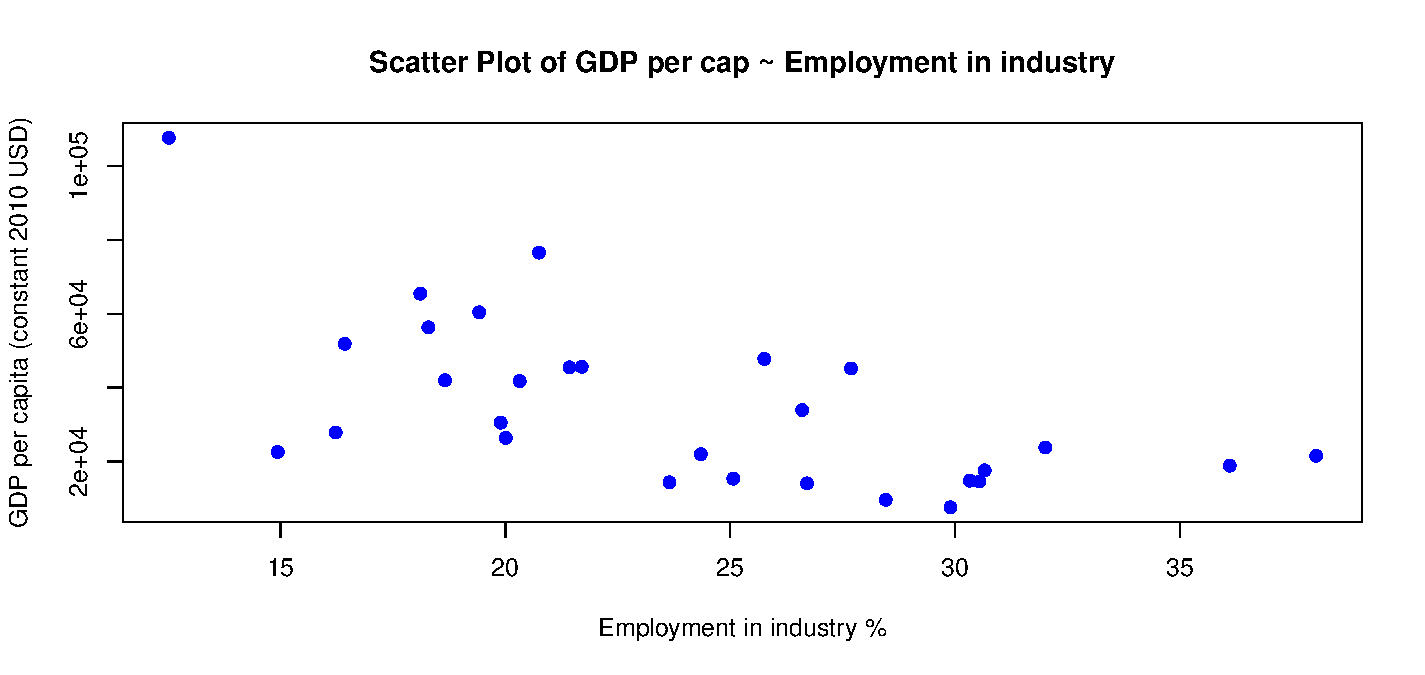
\includegraphics{main_files/figure-latex/mediation_ind-1.pdf}

\begin{table}
\centering
\begin{tabular}{l|r|r|r|r|r|r}
\hline
  & I->D & p-value & I->M & p-value & ACME & p-value\\
\hline
Youth & -2238.58 & 0.0003038 & -0.2893222 & 0.4036032 & 230.4218 & 0.366\\
\hline
Female & -2238.58 & 0.0003038 & -0.1903536 & 0.2552074 & 318.8837 & 0.296\\
\hline
\end{tabular}
\end{table}

\hypertarget{mediation-analysis-gdp-unemp_youth-empl_services}{%
\section{Mediation analysis (GDP, unemp\_youth,
empl\_services)}\label{mediation-analysis-gdp-unemp_youth-empl_services}}

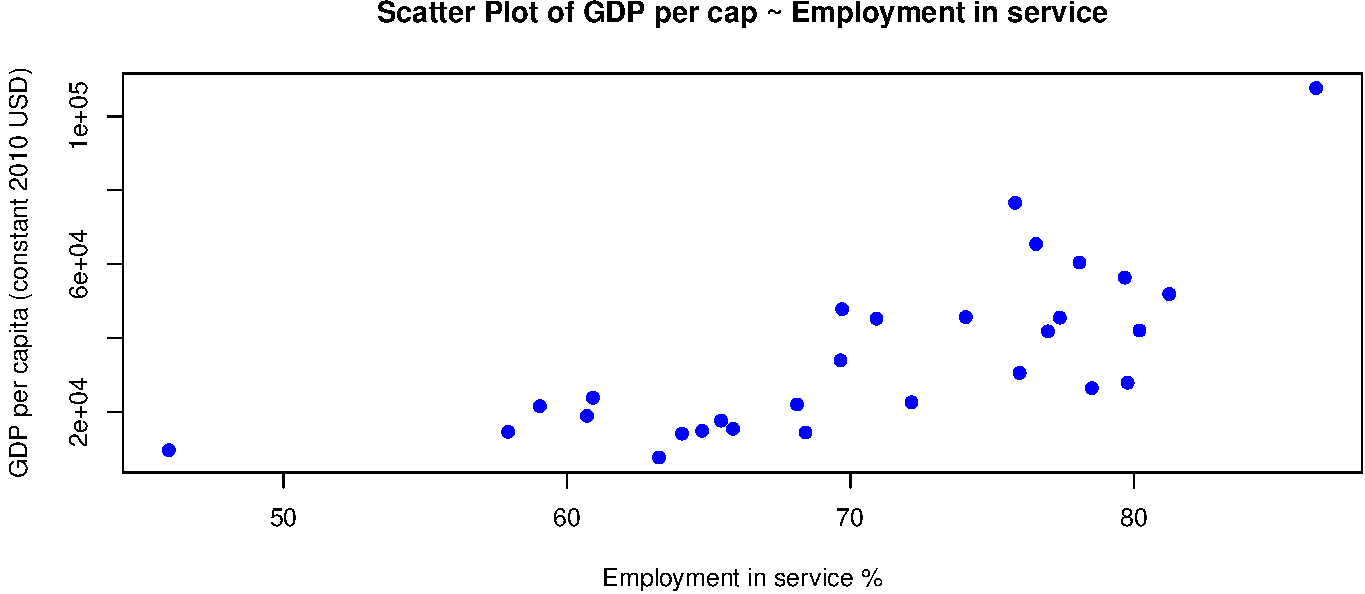
\includegraphics{main_files/figure-latex/mediation_ser-1.pdf}

\begin{table}
\centering
\begin{tabular}{l|r|r|r|r|r|r}
\hline
  & I->D & p-value & I->M & p-value & ACME & p-value\\
\hline
Youth & 1877.316 & 7.1e-06 & -0.0519346 & 0.8352255 & 26.83183 & 0.720\\
\hline
Female & 1877.316 & 7.1e-06 & 0.0199327 & 0.8694560 & -22.56174 & 0.834\\
\hline
\end{tabular}
\end{table}

\hypertarget{sector-analysis-with-wdi-data-2015}{%
\subsection{Sector Analysis with WDI data
(2015)}\label{sector-analysis-with-wdi-data-2015}}

In the remaining part of the project, we consider the effect of
different employment sectors on the GDP. The table below shows the
correlation values for different employment sectors. It can be seen that
employment in agriculture and industry is negatively correlated with GDP
per capita, while employment in services is positively correlated with
the GDP per capita.

\begin{table}
\centering
\begin{tabular}{l|r|r|r|r}
\hline
  & Correlation & Bootstrapping mean & Bootstrapping std. dev. & P-value\\
\hline
Agriculture & -0.507 & -0.512 & 0.0247 & 2e-04\\
\hline
Industry & -0.623 & -0.623 & 0.0429 & 2e-04\\
\hline
Services & 0.730 & 0.731 & 0.0245 & 1e+00\\
\hline
\end{tabular}
\end{table}

As a next step, we would like to use the LinkedIN data to investigate
how migration is impacting the growth of a country. To do so we are
going to use the data provided by a collaboration between World bank and
LinkedIN {[}citation needed{]}. To be consistent in our analysis we will
carry out this analysis filtering only the countries whose WB Region is
marked as ``Europe and Central Asia''.

While to get data on the countries GDP (normalized per capita), and GDP
growth we are going to use the WDI API interface {[}citation needed{]}.
To be consistent with the data provided by LinkedIN we are going to
fetch the data between 2015 and 2019.

Now that we have the data that we need we can merge it in a single
database that shows the migration flux among European countries, and
GDPpc, GDP growth, and unemployment for both the source and destination
countries. Each row contains information about a specific year, about
the migration flux between a base and a target country. The migration
flux is normalized according to the number of LinkedIN users in the base
country. This number is positive when more people are arriving from,
than leaving to the target country, and negative when the opposite
happens.

Now that we have created the dataframe, we can start to investigate the
relationship between the migration to a country and its wealth. The
first step is to actually whether there is a trend in the destination of
the migratory fluxes. To answer this question, Figure
\ref{fig:migration_peryear} (left) plots a country's migration flux as a
function of its GDP, grouped by year. From the plot we have removed
Luxembourg, that is a clear outlier, possibly because of its very small
population. What we note from this plot is that there seems to be a
positive correlation between migration flux and destination country GDP,
suggesting that, as expected, more people tend to emigrate to wealthier
countries, where the quality of life expectancy is higher.

\begin{figure}
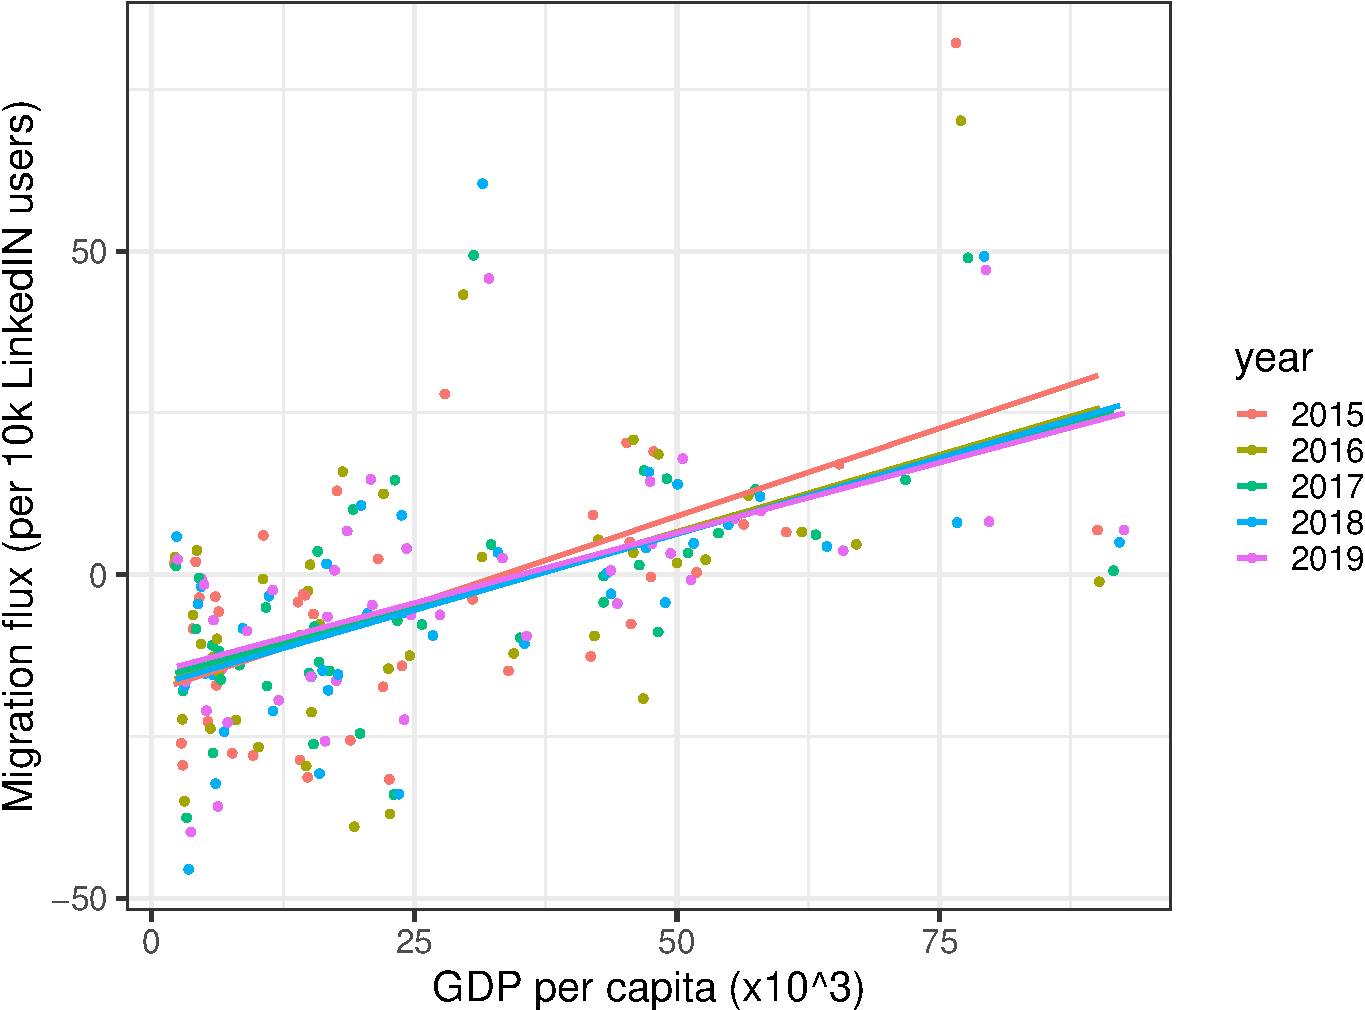
\includegraphics[width=0.5\linewidth]{main_files/figure-latex/migration_peryear-1} 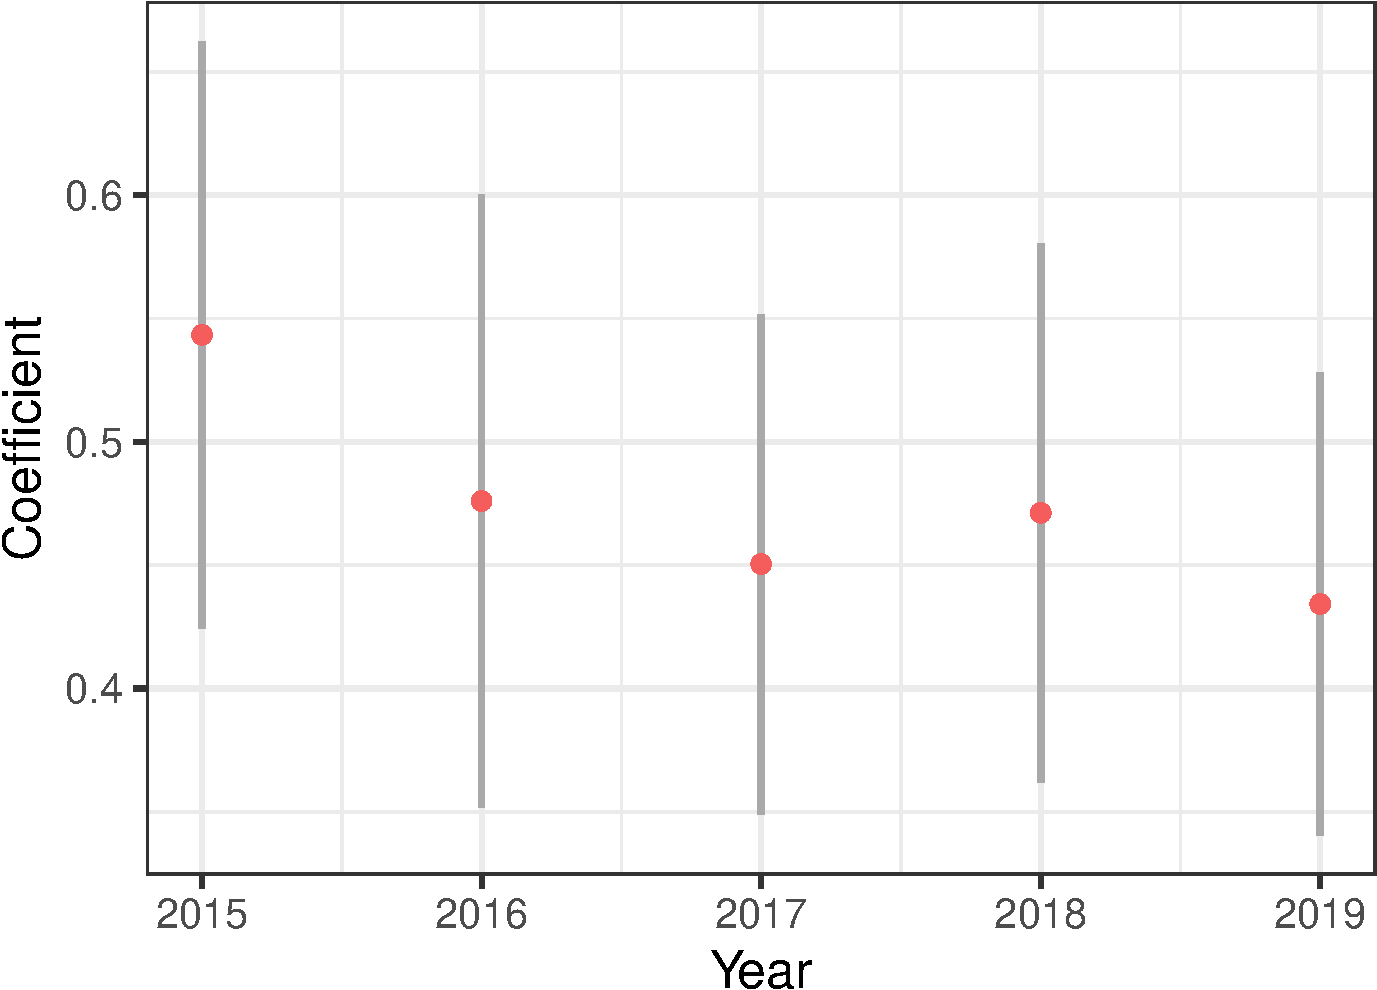
\includegraphics[width=0.5\linewidth]{main_files/figure-latex/migration_peryear-2} \caption{Relation between net flux migration of country X expressed as unit per 10k linkedIN users of that country and the country's GDP per capita. The data are grouped by year, and interpolated by means of linear regression. \label{fig:migration_peryear}}\label{fig:migration_peryear}
\end{figure}

First of all we should check the significance of this result. We can do
so through the p value. The highest value is
\ensuremath{4.6\times 10^{-4}}, which is well below the threshold of
0.05, implying that this correlation is significant. Then, as a next
step, we could estimate the quality of the fit through the
R\textsuperscript{2} statistic individually for each year. This is in
the range of 0.27 for the year 2016 to 0.35 for the year 2019. Meaning
that whilst the fit is not perfect, it can explain more than the 25\% of
the data variance. Moreover, it can be noted how the coefficient of the
fix seems to be decreasing with time. To have a better picture, Figure
\ref{fig:migration_peryear} (right) shows the coefficient together with
a 1 std.err. per each year. From such figure we can evince that the
decreasing trend seems to be within the 1 std.err. range, making it
harder to distinguish from normal fluctuations. More data points will
definitely be helpful in clearing up the picture.

To get more insights of the fit, we can plot the histogram of the
residuals for the years with the best and worst fit, as shown in Figure
\ref{fig:residuals_hist}. As expected we can see that a better fit
corresponds to less spread in the histogram of residuals.

\begin{figure}
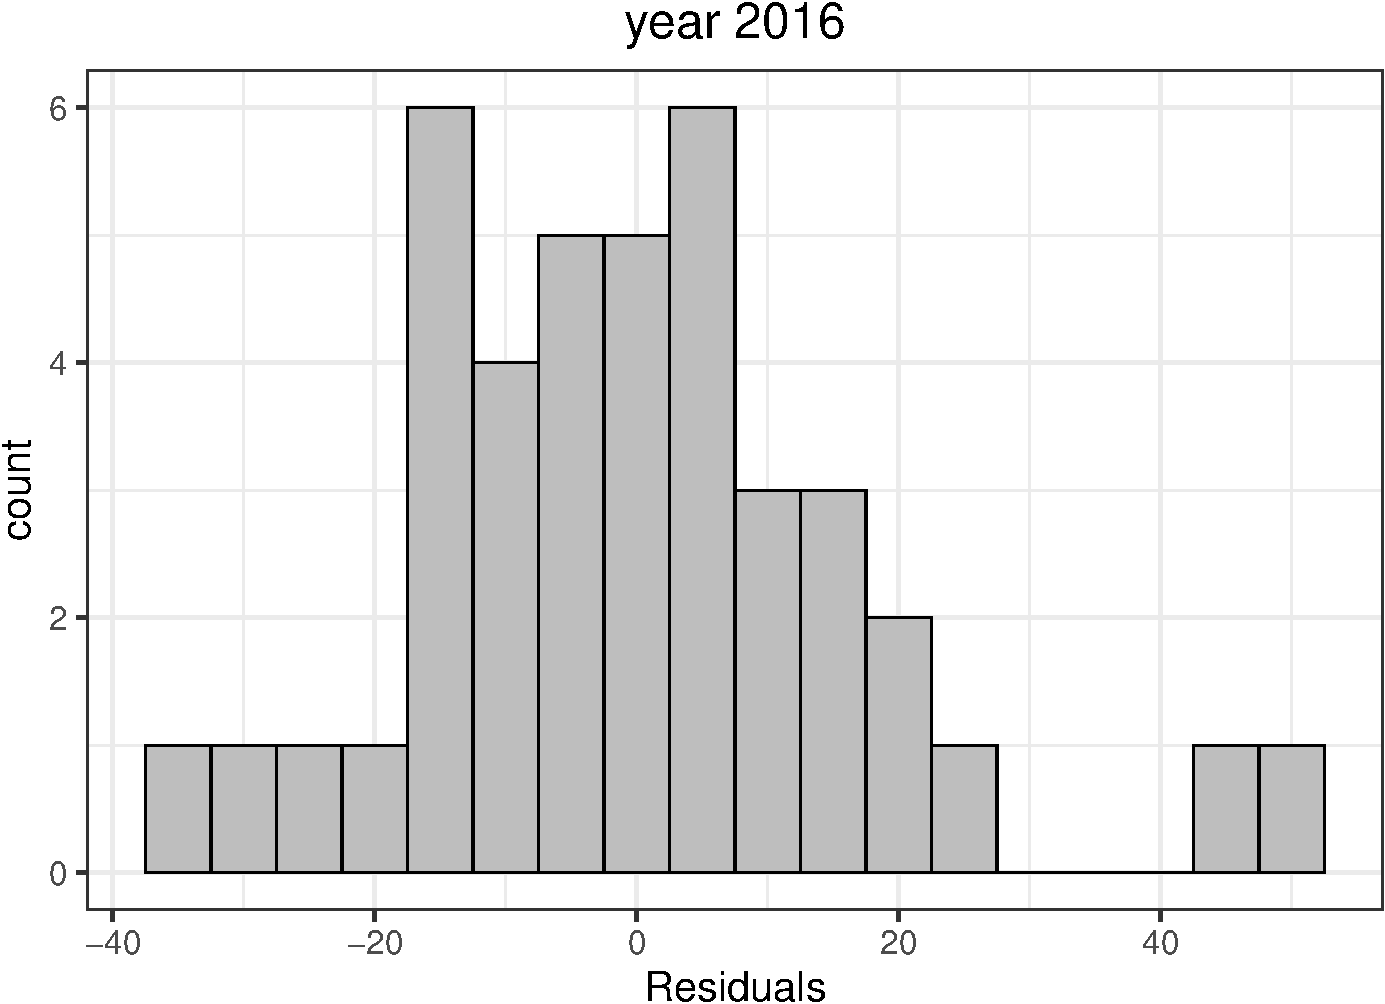
\includegraphics[width=0.5\linewidth]{main_files/figure-latex/residuals_hist-1} 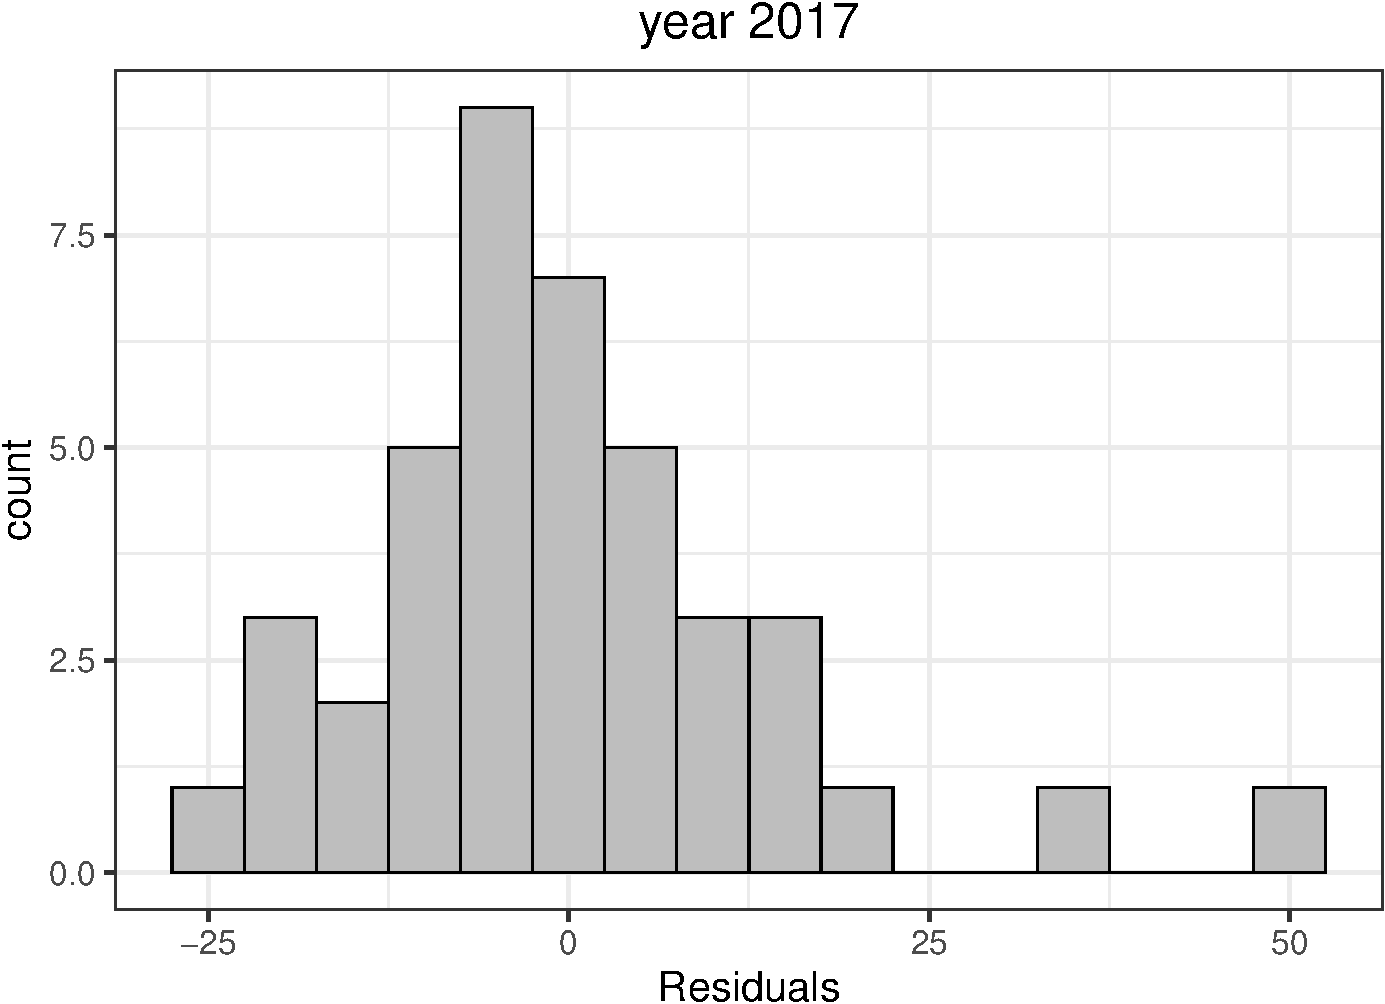
\includegraphics[width=0.5\linewidth]{main_files/figure-latex/residuals_hist-2} \caption{Histograms of residuals for the year with worst fit (left) and best fit (right). \label{fig:residuals_hist}}\label{fig:residuals_hist}
\end{figure}

Even though the dataset is quite small, since it includes one point per
country per year, we can try to perform a bootstrap anaysis to check
whether our data contains some bias. For simplicity, we will only
perform this analysis on one single year; to be consistent, we will keep
using the year 2015. Then, the bootstrap analysis will compute the
linear regression coefficient over a limited dataset that allows
repetitions. Here we have performed it for 10000 replicates, and the
histogram showing the variation of interpolating coefficients is shown
in Figure \ref{fig:bootModel}.

\begin{figure}
\centering
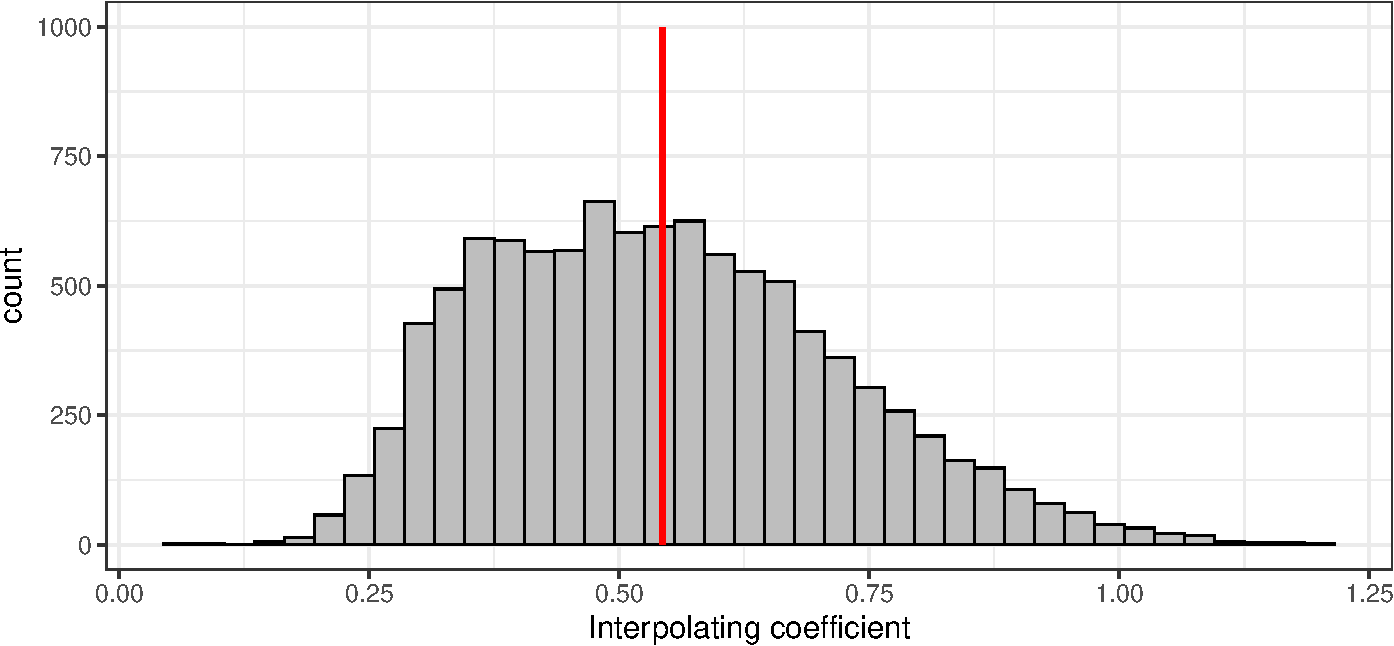
\includegraphics{main_files/figure-latex/bootModel-1.pdf}
\caption{Histograms of coefficients when performing a bootstrap analysis
of migration flux vs GDP per capita of year 2015, with R = 10000. In red
is depicted the interpolating coefficient of the original dataset.
\label{fig:bootModel}}
\end{figure}

From this histogram we can first of all note how the original
coefficient is at the center of the gaussian, and how in 100\% of cases,
the interpolating coefficient is greater than 0. Thus we can comfortably
state that there is a correlation between the migration flux and GDPpc
of a country. At the same time, however, the distribution is quite wide
spread, with a standard deviation of 0.17. Hence, whilst we can state
the presence of a correlation, from this analysis alone, it is hard to
quantify the strength of such correlation, as the addition of more data
can significantly alter the results.

We have shown how wealthier countries tend to benefit from a larger
working migration flux, it is interesting to study whether these
countries are benefiting from this larger migratory flux. To do so we
can plot the GDP growth as a function of the migration flux of a
country. Again, as a first step, we will perform this analysis grouping
the countries by year, and, as in the previous analysis, we will exclude
Luxembourg, as it is a clear outlier. The results are shown in Figure
\ref{fig:growthVSmigration}.

\begin{figure}
\centering
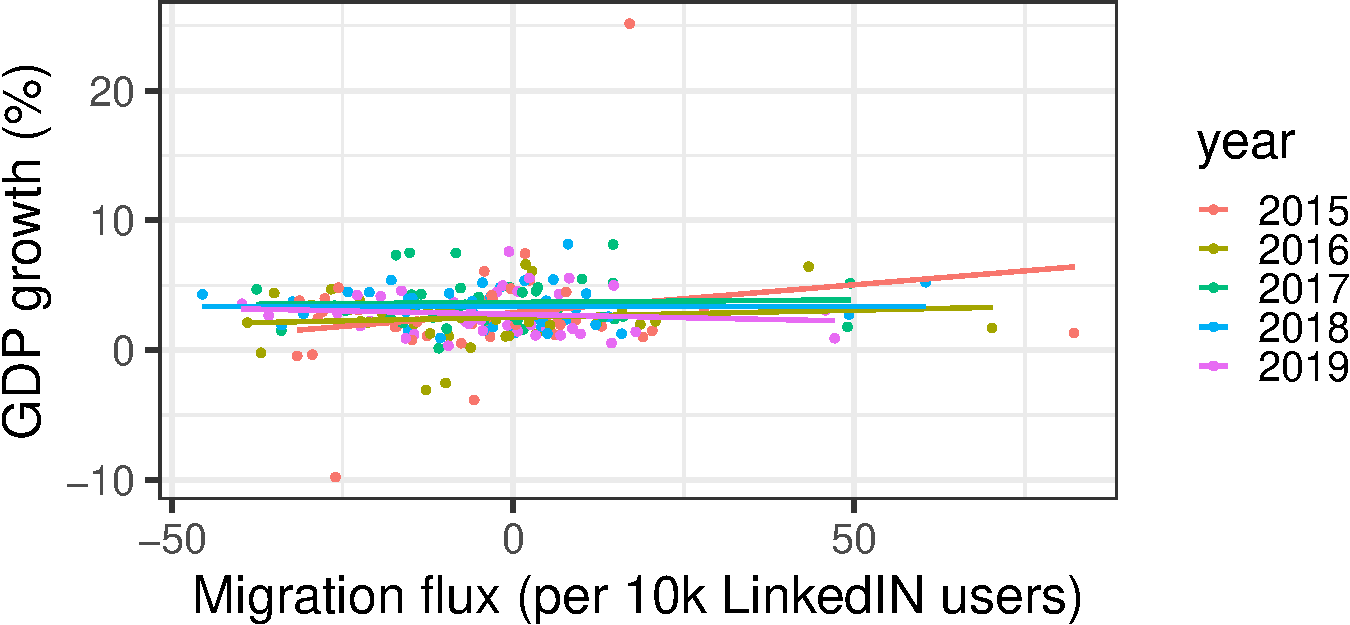
\includegraphics{main_files/figure-latex/growthVSmigration-1.pdf}
\caption{Plot relating the GDP growth of a country to the migrating flux
(per 10k of linkedIN users), for the years 2015 to 2019. The points are
fitted through the linear regression method.
\label{fig:growthVSmigration}}
\end{figure}

This plot shows how there does not seem to be any correlation between
GDP growth and migration, in fact the interpolating curves are very
flat, and have very large residuals. This is confirmed by the p values,
as they are all higher than 0.22. Moreover, the R\textsuperscript{2}
statistics are very low, up to 0.04. From this it is possible to
conclude that, with only increase of production in mind, it should not
be a country's first priority to be more appealing to foreign workers.

\hypertarget{industries-preferred-by-migratory-workers}{%
\subsection{Industries preferred by migratory
workers}\label{industries-preferred-by-migratory-workers}}

To have a deeper look at how migration imapcts the growth of a country,
we can also investigate whether a higher migration influx correlates to
a larger growth of specific industries. To do so we are going to use
again the linkedIN data that depicts the net gain (or loss) of members
from (or to) a foreign country, for a specific industry, normalized to
the number of linkedIN users, in that industry, in that country. These
industries are gouped in different ISIC sections {[}citation needed{]}.
The aim of this section is to verify whether net migration flux
correlates to a larger growth of one of these sections. We are going to
carry on this analysis for only one year, that is 2015.

Figure \ref{fig:growthVSmigration2} (left) depicts the data points
grouped per ISIC section index, fitted through linear regression. Then,
Figure \ref{fig:growthVSmigration2} (right) shows the slope of such
interpolations, together with 1 std. error.

\begin{table}

\caption{\label{tab:growthVSmigration2}R squared and p values for the fit of industry growth due to migration vs migration flux.    \label{tab:industryGrowth}}
\centering
\begin{tabular}[t]{lllllllllllll}
\toprule
isic\_sector & A & B & C & D & F & G & H & I & K & N & Q & R\\
P value & 4.10e-02 & 4.14e-02 & 5.57e-06 & 5.02e-03 & 7.75e-03 & 1.52e-06 & 9.94e-06 & 2.67e-05 & 5.54e-04 & 3.25e-04 & 6.26e-03 & 4.22e-07\\
R\textasciicircum{}2\textasciicircum{} & 0.472 & 0.131 & 0.584 & 0.494 & 0.220 & 0.610 & 0.549 & 0.499 & 0.315 & 0.451 & 0.293 & 0.748\\
\bottomrule
\end{tabular}
\end{table}

\begin{figure}
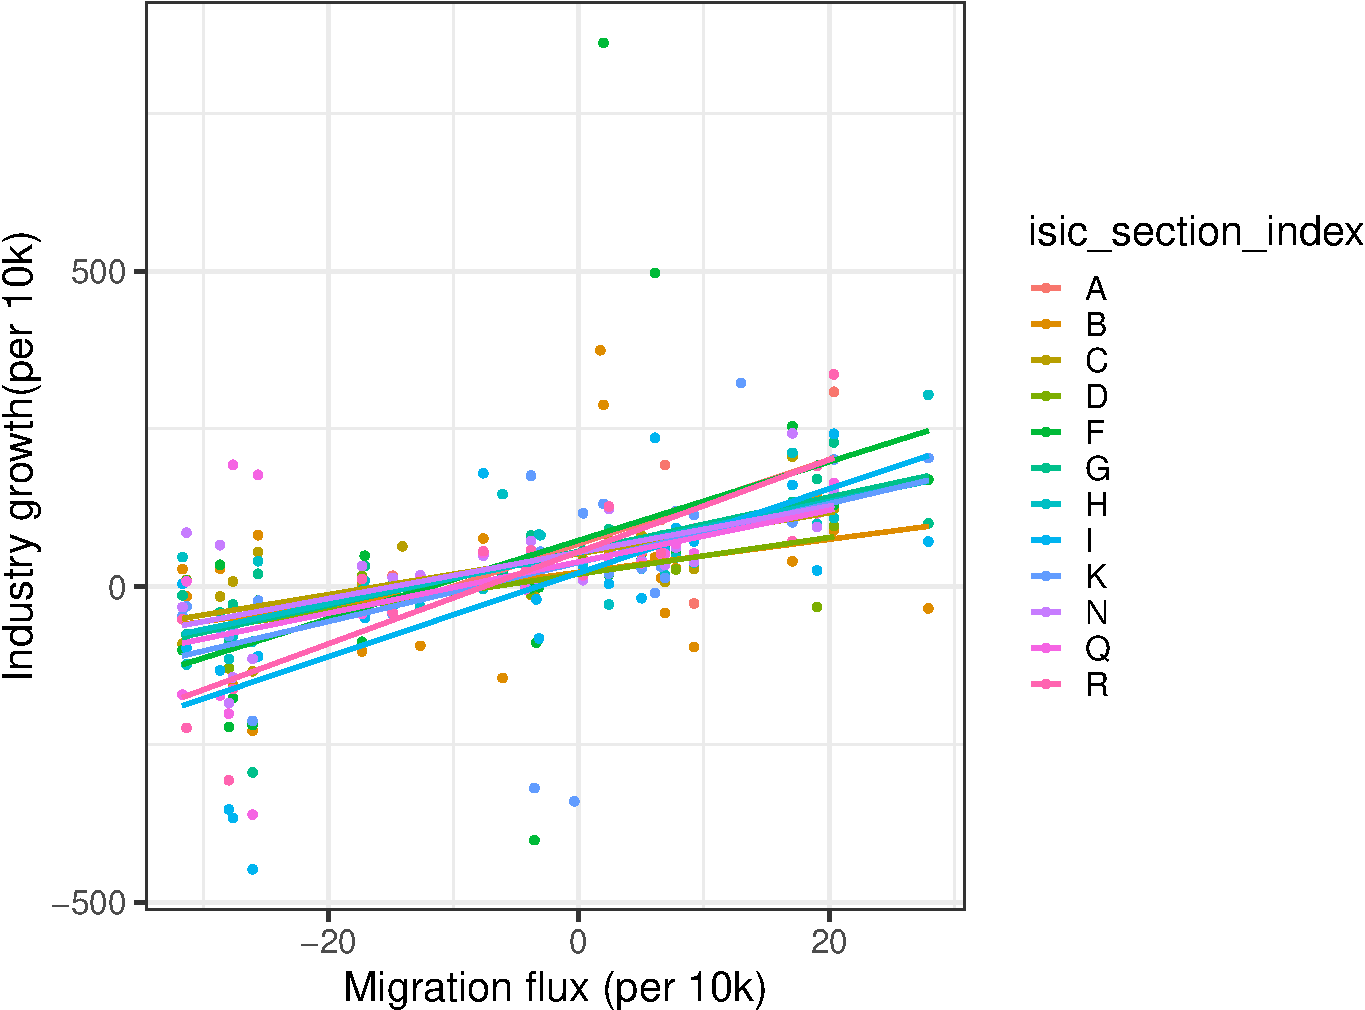
\includegraphics[width=0.5\linewidth]{main_files/figure-latex/growthVSmigration2-1} 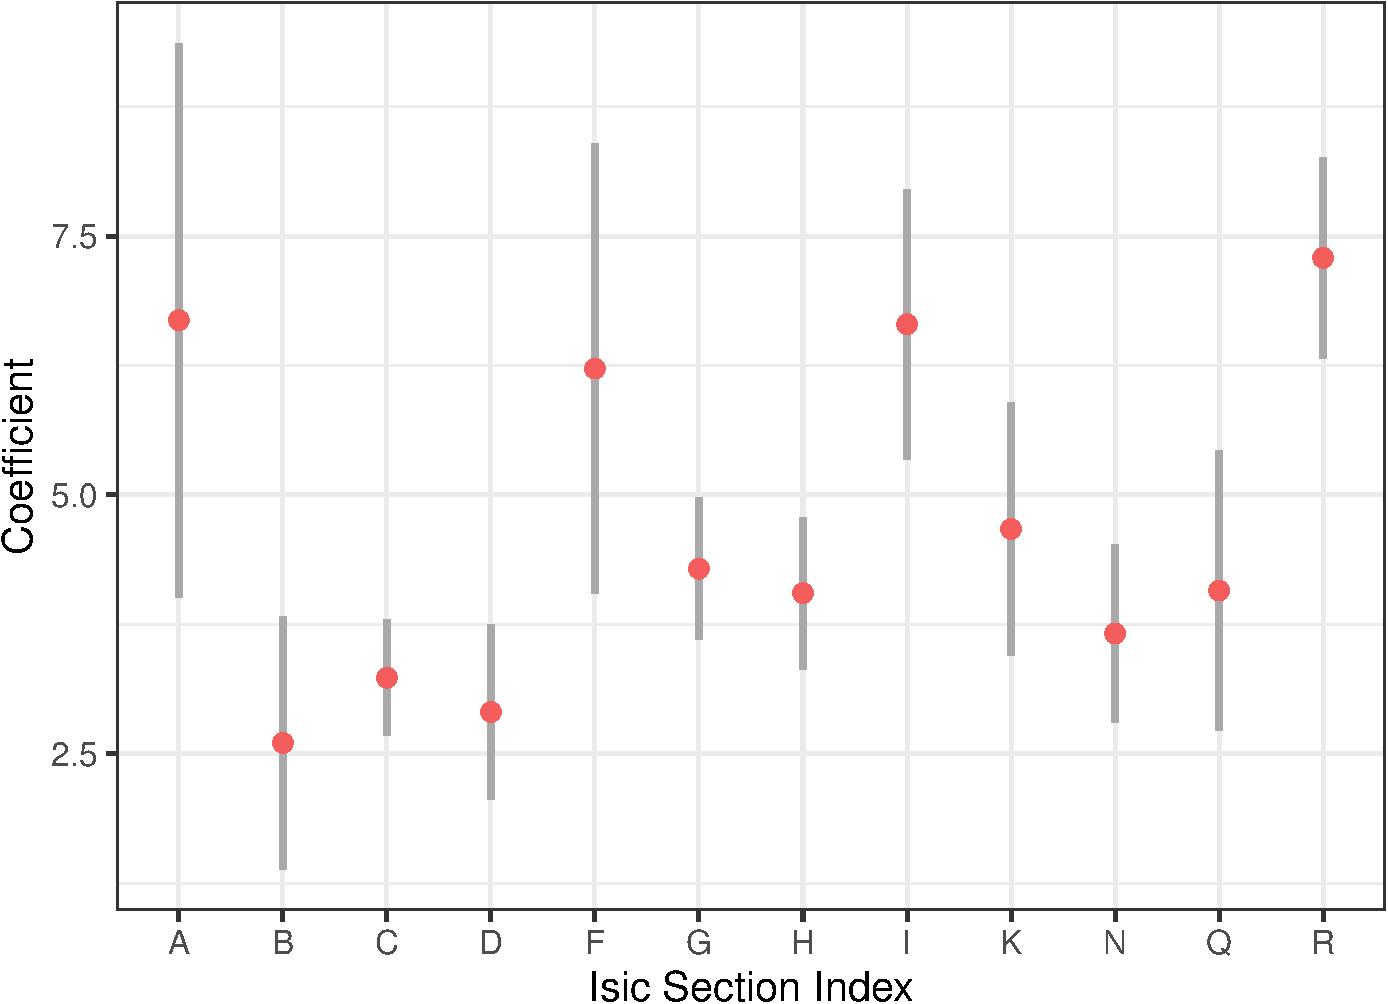
\includegraphics[width=0.5\linewidth]{main_files/figure-latex/growthVSmigration2-2} \caption{Industry growth due to migration as a function of net migration in the year 2019. \label{fig:growthVSmigration2}}\label{fig:growthVSmigration2}
\end{figure}

We can notice how the B, C and D sectors are lower than the others.
These are Quarrying, Manufacturing and Energy respectively. On the other
side, there is a stronger correlation with the sections F, I, R, which
are Construction, Accomodation and Arts \& Entertainment respectively.
It is also important to notice that the industry growth due to
foreigners can go up to a non-negligible 3\%. With this in mind,
incentivating a working migratory flux can help a country in develop
certain industry sectors, that would otherwise be less populated.

The p values and R\textsuperscript{2} values are shown in table
\ref{tab:industryGrowth}. All p values are below the 0.05
threshold.Moreover, the sectors A and F have a very large std.err.,
meaning that there is probably more variability across the countries,
and a correlation with the migration flux alone is not enough.

\hypertarget{limitations}{%
\subsection{Limitations}\label{limitations}}

When doing such an analysis is it also important to identify where the
limitations are. The first, most obvious one, is that this data has been
normalized to the number of LinkedIN users for each country. We could
not cross-validate this data with other employment datasets. Still,
according to the source, this data has already been validated with 23
other external datasets. Moreover, these data do not include any
differentiation such as gender or age. It would be interesting to
investigate how migration fluxes differ for these categories.

\end{document}
